\begin{figure}[H]
	\centering
	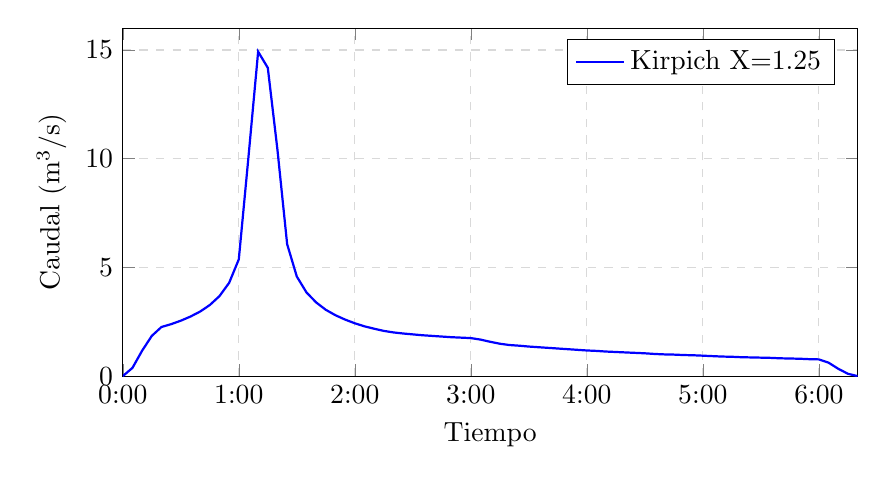
\begin{tikzpicture}
		\begin{axis}[
			width=0.9\textwidth,
			height=6cm,
			xlabel={Tiempo},
			ylabel={Caudal (m$^3$/s)},
			xmin=0,
			xmax=380,
			ymin=0,
			ymax=16,
			grid=major,
			grid style={dashed, gray!30},
			legend pos=north east,
			xtick={0, 60, 120, 180, 240, 300, 360},
			xticklabels={0:00, 1:00, 2:00, 3:00, 4:00, 5:00, 6:00},
			]
		% Kirpich X=1.25
		\addplot [
		blue,
		thick,
		solid,
		] coordinates {
				(0, 0.00) (5, 0.38) (10, 1.17) (15, 1.85) (20, 2.26)
				(25, 2.39) (30, 2.55) (35, 2.74) (40, 2.97) (45, 3.27)
				(50, 3.68) (55, 4.29) (60, 5.37) (65, 10.08) (70, 14.92)
				(75, 14.18) (80, 10.40) (85, 6.07) (90, 4.58) (95, 3.85)
				(100, 3.39) (105, 3.05) (110, 2.80) (115, 2.60) (120, 2.43)
				(125, 2.29) (130, 2.18) (135, 2.08) (140, 2.01) (145, 1.96)
				(150, 1.92) (155, 1.88) (160, 1.85) (165, 1.82) (170, 1.79)
				(175, 1.77) (180, 1.75) (185, 1.68) (190, 1.58) (195, 1.49)
				(200, 1.43) (205, 1.40) (210, 1.36) (215, 1.33) (220, 1.30)
				(225, 1.27) (230, 1.24) (235, 1.21) (240, 1.18) (245, 1.16)
				(250, 1.13) (255, 1.11) (260, 1.09) (265, 1.07) (270, 1.05)
				(275, 1.02) (280, 1.00) (285, 0.99) (290, 0.97) (295, 0.96)
				(300, 0.94) (305, 0.92) (310, 0.90) (315, 0.89) (320, 0.87)
				(325, 0.86) (330, 0.85) (335, 0.84) (340, 0.82) (345, 0.81)
				(350, 0.80) (355, 0.78) (360, 0.77) (365, 0.62) (370, 0.34)
				(375, 0.11) (380, 0.00)
		};
		\addlegendentry{Kirpich X=1.25}

		\end{axis}
	\end{tikzpicture}
	\caption{Hidrograma - Kirpich + GZ $T_r$=25 años ($Q_p$=14.920 m$^3$/s)}
	\label{fig:hydro_kirpich_gz_Tr25_X125}
\end{figure}
